% Created 2020-11-13 Fri 23:29
% Intended LaTeX compiler: pdflatex
\documentclass[11pt]{article}
\usepackage[utf8]{inputenc}
\usepackage[T1]{fontenc}
\usepackage{graphicx}
\usepackage{grffile}
\usepackage{longtable}
\usepackage{wrapfig}
\usepackage{rotating}
\usepackage[normalem]{ulem}
\usepackage{amsmath}
\usepackage{textcomp}
\usepackage{amssymb}
\usepackage{capt-of}
\usepackage{hyperref}
\usepackage[newfloat]{minted}
\usepackage{caption}
\author{Yi Zhang}
\date{\today}
\title{Compare mrgsolve and Torsten for EVID=4}
\hypersetup{
 pdfauthor={Yi Zhang},
 pdftitle={Compare mrgsolve and Torsten for EVID=4},
 pdfkeywords={},
 pdfsubject={},
 pdfcreator={Emacs 27.1 (Org mode 9.1.4)}, 
 pdflang={English}}
\begin{document}

\maketitle

\section{Background}
\label{sec:orgdb707e1}
This report summarizes steps to simulate a reset \& dose(EVID=4) event
using \texttt{mrgsolve} and \texttt{Torsten}.

\section{\texttt{Torsten} model}
\label{sec:org2a6b3d0}
First download the repo with
\begin{minted}[breaklines=true,fontsize=\footnotesize,breakanywhere=true]{bash}
git clone -b reset_test git@github.com:metrumresearchgroup/Torsten.git
\end{minted}
Then make the model
\begin{minted}[breaklines=true,fontsize=\footnotesize,breakanywhere=true]{bash}
make -j4 examples/pk2cpt_reset/reset
\end{minted}
To run the model, do
\begin{minted}[breaklines=true,fontsize=\footnotesize,breakanywhere=true]{bash}
cd examples/pk2cpt_reset/
./reset sample algorithm=fixed_param num_warmup=1 num_samples=1 data file=reset.data.json init=reset.init.R
\end{minted}
The above run produces deterministic ODE solutions for
a two-compartment PK model based on
parameters in \texttt{reset.init.R} and data \texttt{reset.data.json}.

One can use \texttt{cmdstanr} package in \texttt{R} to extract the concentration in central compartment
\begin{minted}[breaklines=true,fontsize=\footnotesize,breakanywhere=true]{r}
fit <- cmdstanr::read_cmdstan_csv("output.csv", variables=c("cHat"))
draws <- fit$post_warmup_draws
torsten.cp <- as.numeric(as.data.frame(draws)[1,])
\end{minted}

\section{\texttt{mrgsolve} model}
\label{sec:org88c1f76}
\begin{minted}[breaklines=true,fontsize=\footnotesize,breakanywhere=true]{r}
library("mrgsolve")

code <- '
$PARAM CL = 5, Q = 8, V2 = 20, V3 = 70, KA = 1.2

$CMT GUT CENT PERI

$GLOBAL
#define CP (CENT/V2)

$PKMODEL ncmt = 2, depot = TRUE

## $SIGMA 0.01  // variance

$TABLE
capture DV = CP * exp(EPS(1));

$CAPTURE CP
'

mod <- mcode("accum", code) %>% Req(CP) %>% update(end=480,delta=0.1)

data <- rbind(data.frame("time" = 0, "amt" = 10000, "ii" = 24, "addl"=1, cmt=1, evid=1),data.frame("time" = 18, "amt" = 8000, "ii"=0, "addl"=0, cmt=1, evid=4))
data$ID=1
mrgsol <- mod %>% data_set(data) %>% mrgsim(end=50)
\end{minted}

\section{Compare results}
\label{sec:org71d43be}
\begin{minted}[breaklines=true,fontsize=\footnotesize,breakanywhere=true]{r}
## first we import Torsten's data file
torsten.data <- jsonlite::read_json("reset.data.json", simplifyVector = TRUE)

## plot
par(mfrow=c(1,2))
plot(torsten.data$time, torsten.cp, type="l", col="red")
plot(mrgsol$time, mrgsol$CP, type="l", col="green")
## or overlay with
## lines(res$time,res$CP,col="green")
\end{minted}

\begin{figure}[htbp]
\centering
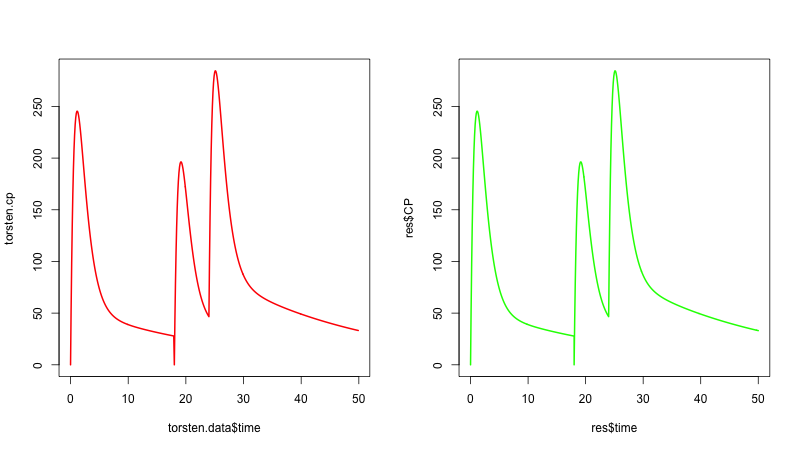
\includegraphics[width=\textwidth]{./reset_compare.png}
\caption{Compare \texttt{Torsten} (left) \& \texttt{mrgsolve} (right) central compartment solution}
\end{figure}
\end{document}
